

本小节主要做的实验为完成在软件上书写完成时钟分频代码以及做初步验证，即实验目的为：
\begin{enumerate}
    \item 以实验平台为基础，了解并熟悉现代信号处理电路的电路构造；
    \item 熟悉使用 IP 核的具体流程；
    \item 熟悉时钟分频的实现原理；
    \item 熟悉使用 Vivado 进行硬件开发的步骤，了解仿真如何在Vivado进行仿真。
\end{enumerate}

\subsection{实验原理}


\subsubsection{偶数分频（占空比50\%）}


在输入时钟的驱动下，一次输出翻转只对应
$0\rightarrow 1$ 或 $1\rightarrow 0$，
两次翻转才构成一个完整周期。

因此，只需要通过计数器数拍，并在计满半个输出周期时
翻转输出，即可实现偶数分频。

例如，每经过 $5$ 个输入时钟周期翻转一次输出，
则一个完整的输出周期包含 $10$ 个输入时钟周期，
因此实现了 $10$ 分频。

设分频系数为偶数 $N$，则有
\[
T_{\mathrm{out}} = N T_{\mathrm{in}},
\qquad
f_{\mathrm{out}} = \frac{f_{\mathrm{in}}}{N}.
\]

输出每隔 $\frac{N}{2}$ 个输入时钟周期翻转一次，即
\[
T_{\mathrm{toggle}} = \frac{N}{2}T_{\mathrm{in}}.
\]

对应到代码上（以 6 分频为例），则需要我们
复位解除后，计数器从 $0$ 开始计数。
输入时钟上升沿到来时，执行如下动作：

\begin{table}[H]
  \centering
  \caption{6 分频的计数与翻转过程}
  \begin{tabularx}{\textwidth}{ccX}
    \toprule
    输入上升沿 & 沿到来前的计数值 & 该沿执行的动作 \\
    \midrule
    第一个 & 0 & 计数值更新为 1。 \\
    第二个 & 1 & 计数值更新为 2。 \\
    第三个 & 2 & 已计满 3 拍，输出翻转，同时计数器清零。 \\
    \bottomrule
  \end{tabularx}
\end{table}

因此，当计数器从 $0$ 开始计数时，可使用以下条件判断翻转时机：
\[
\boxed{\texttt{count} = \frac{N}{2}-1}
\]

对于 $6$ 分频，判断阈值为
\[
\texttt{count} = \frac{6}{2}-1 = 2.
\]

\subsubsection{奇数分频（ 50\% 占空比）}

如果只使用输入时钟的上升沿，或者只使用输入时钟的下降沿，
则只能按照整数个输入时钟周期安排输出的高、低电平持续时间。

当分频系数为奇数时，若要求占空比为 $50\%$，
则输出高电平与低电平的持续时间均为
\[
T_{\mathrm{high}} = T_{\mathrm{low}}
= \frac{N}{2}T_{\mathrm{in}}.
\]

由于 $N$ 为奇数，$\frac{N}{2}$ 不是整数，
因此需要能够表示半个输入时钟周期的方法。

例如，$5$ 分频且占空比为 $50\%$ 时，需要满足
\[
T_{\mathrm{high}} = T_{\mathrm{low}}
= 2.5T_{\mathrm{in}}.
\]

一种方法是同时利用输入时钟的上升沿和下降沿。
当输入时钟占空比为 $50\%$ 时，相邻上升沿与下降沿之间
恰好相隔半个输入时钟周期。

可以将最终输出拆分为两个信号 $A$、$B$ 的或运算。
其中，$B$ 相对于 $A$ 延迟半个输入时钟周期。

以 5 分频为例的波形组合，以输入时钟周期为时间单位，其高电平区间如下：

\begin{table}[H]
  \centering
  \caption{5 分频的高电平区间组合}
  \begin{tabular}{cc}
    \toprule
    信号 & 高电平区间 \\
    \midrule
    $A$ & $0 \sim 2$ 拍 \\
    $B$ & $0.5 \sim 2.5$ 拍 \\
    $A \lor B$ & $0 \sim 2.5$ 拍 \\
    \bottomrule
  \end{tabular}
\end{table}

两个信号的高电平区间在中间部分重叠，
只在起始与结束处各相差半拍。
通过或运算，合成信号的高电平持续时间为
\[
T_{\mathrm{high}} = \frac{N}{2}T_{\mathrm{in}}.
\]

合成输出可以表示为
\[
\boxed{\texttt{clk\_out} = A \lor B}
\]

在代码实现上：
分别利用上升沿和下降沿更新信号 $A$、$B$，
并提出在以下计数条件下翻转：
\[
\texttt{counter} = \frac{N-1}{2}-1.
\]


\subsubsection{时钟IP核}
时钟IP虽然可以提供准确的时钟，但是需要一段时间来建立稳定的时钟关系。
当状态信号$ locked = 1 $时，时钟才正式准备好。


\subsubsection{testbench仿真平台}

仿真时长需要根据待验证信号的周期合理设置。

如果仿真时间不足以覆盖待验证信号的变化过程，
就可能无法观察到预期现象。因此，应保证仿真时间能够覆盖
复位过程以及若干个完整的输出时钟周期。

\subsection{实验过程}
实验步骤如下：
\begin{enumerate}
    \item 新建工程：器件型号按实验箱 FPGA（XC7K410T-2FFG900）选择；
    \item 配置 Clocking Wizard IP：输入 25MHz，倍频输出 100MHz、200MHz（10MHz 可由 IP 核输出或分频模块生成）；
    \item 编写分频模块与顶层文件：100MHz→20MHz、10MHz→1KHz（计数器翻转法，参考讲义代码框架）；
    \item 添加约束文件：时钟约束 \texttt{create\_clock} + 引脚约束 \texttt{PACKAGE\_PIN}（25M 时钟引脚 C25，LVCMOS33）；
    \item 行为仿真：验证分频比与占空比（注意仿真时长是否足够）；
\end{enumerate}

预期可以观察到IP核产生的100MHz，20MHz，1KHz时钟信号，以及分频模块产生的100MHz，20MHz，1KHz时钟信号的频率均正确，占空比均为50\%。

一些实验过程图展示：

\begin{figure}[H]
    \centering
    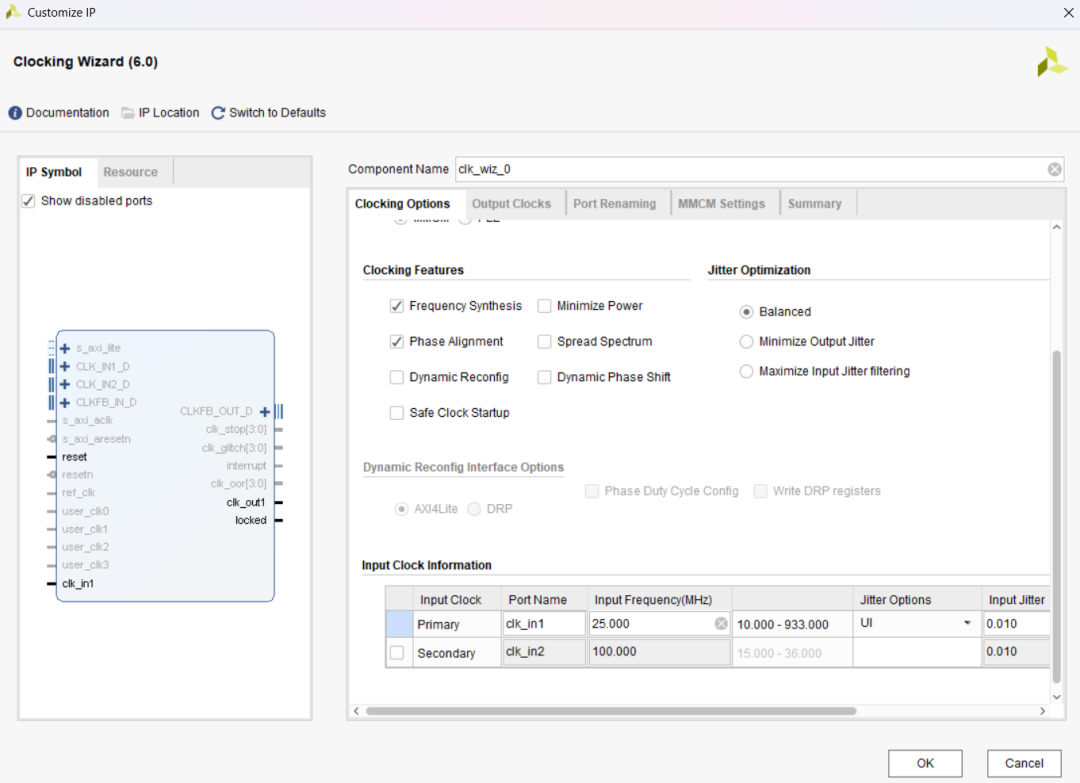
\includegraphics[width=0.75\textwidth]{figures/clk_in.png}\\[0.5em]
    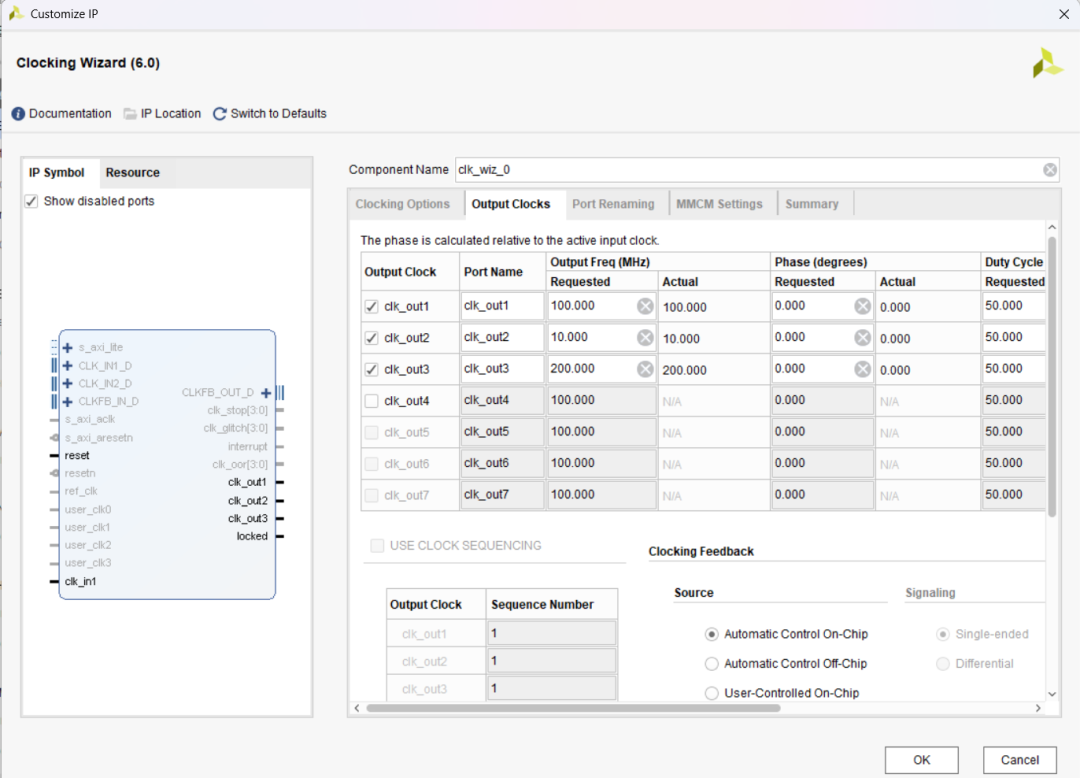
\includegraphics[width=0.75\textwidth]{figures/clk_out.png}
    \caption{Clocking Wizard IP 配置：上图为输入时钟 25MHz，下图为输出时钟 100MHz、10MHz、200MHz}
    \label{fig:clk_wiz}
\end{figure}

% \subsection{预期现象}
% \input{imag.tex}

用到的代码：

\begin{lstlisting}[style=vcode, caption={奇数分频模块（5 分频，占空比 50\%）}, label={lst:clk_div_odd}]
`timescale 1ns / 1ps

module clk_div_odd #(
    parameter DIV_FACTOR = 5
)(
    input wire clk_in,
    input wire sys_rstn,
    output wire clk_out
);

reg [31:0] counter;
reg clk_pos;
reg clk_neg;

always @(posedge clk_in or negedge sys_rstn) begin
    if (!sys_rstn) begin
        counter <= 0;
        clk_pos <= 0;
    end
    else begin
        if (counter == DIV_FACTOR - 1)
            counter <= 0;
        else
            counter <= counter + 1;

        clk_pos <= (counter < (DIV_FACTOR - 1) / 2);
    end
end

always @(negedge clk_in or negedge sys_rstn) begin
    if (!sys_rstn)
        clk_neg <= 0;
    else
        clk_neg <= clk_pos;
end

assign clk_out = clk_pos | clk_neg;

endmodule
\end{lstlisting}

% 【代码2】


\begin{lstlisting}[style=vcode, caption={偶数分频（占空比50\%）}, label={lst:clk_div_even}]
module clk_div_even #
(
    parameter DIV_FACTOR = 10
)
(
    clk_in,
    sys_rstn,
    clk_out
);

input clk_in;
input sys_rstn;
output reg clk_out;

reg [15:0] counter;

localparam COUNT = (DIV_FACTOR >> 1);

always @(posedge clk_in or negedge sys_rstn) begin
    if (!sys_rstn) begin
        counter <= 0;
        clk_out <= 0;
    end
    else if (counter == COUNT - 1) begin
        clk_out <= ~clk_out;
        counter <= 0;
    end
    else begin
        counter <= counter + 1;
    end
end

endmodule
\end{lstlisting}



\begin{lstlisting}[style=vcode, caption={约束文件}]
# 25MHz board clock input
set_property PACKAGE_PIN C25 [get_ports sys_clk]

# Input I/O standard
set_property IOSTANDARD LVCMOS33 [get_ports sys_clk]

# Clock period: 40ns = 25MHz
create_clock -name sys_clk -period 40.000 [get_ports sys_clk]

\end{lstlisting}


\subsection{实验结果}
% 【100_10_20MHz】
% 【100_20_10_1k】

